\UseRawInputEncoding
\documentclass[12pt]{article}
\title{ECE 141 Homework 4}
\usepackage{subcaption}
\author{Lawrence Liu}
\usepackage{graphicx}
\usepackage{amsmath}
\usepackage{placeins}
\newcommand{\Laplace}{\mathscr{L}}
\setlength{\parskip}{\baselineskip}%
\setlength{\parindent}{0pt}%
\usepackage{xcolor}
\usepackage{listings}
\definecolor{backcolour}{rgb}{0.95,0.95,0.92}
\usepackage{amssymb}
\lstdefinestyle{mystyle}{
    backgroundcolor=\color{backcolour}}
\lstset{style=mystyle}

\begin{document}
\maketitle
\subsection*{Problem 5.5}
\subsection*{(c)}
$L(s)$ has zeros at $\frac{-2\pm j2\sqrt{7}}{2}$, and poles at $0$ and $\frac{-2\pm j6}{2}$, therefore we have $\alpha=0$
$\phi_{1}=180^{\circ}$, 
And the departure angle for poles $-1\pm3j$ is $\pm161.565^{\circ}$, And the arival angle for the zeros $-1\pm\sqrt{7}j$ is $\pm200^{\circ}$\\\\
Therefore the sketch fo the root locus looks like the following
\\
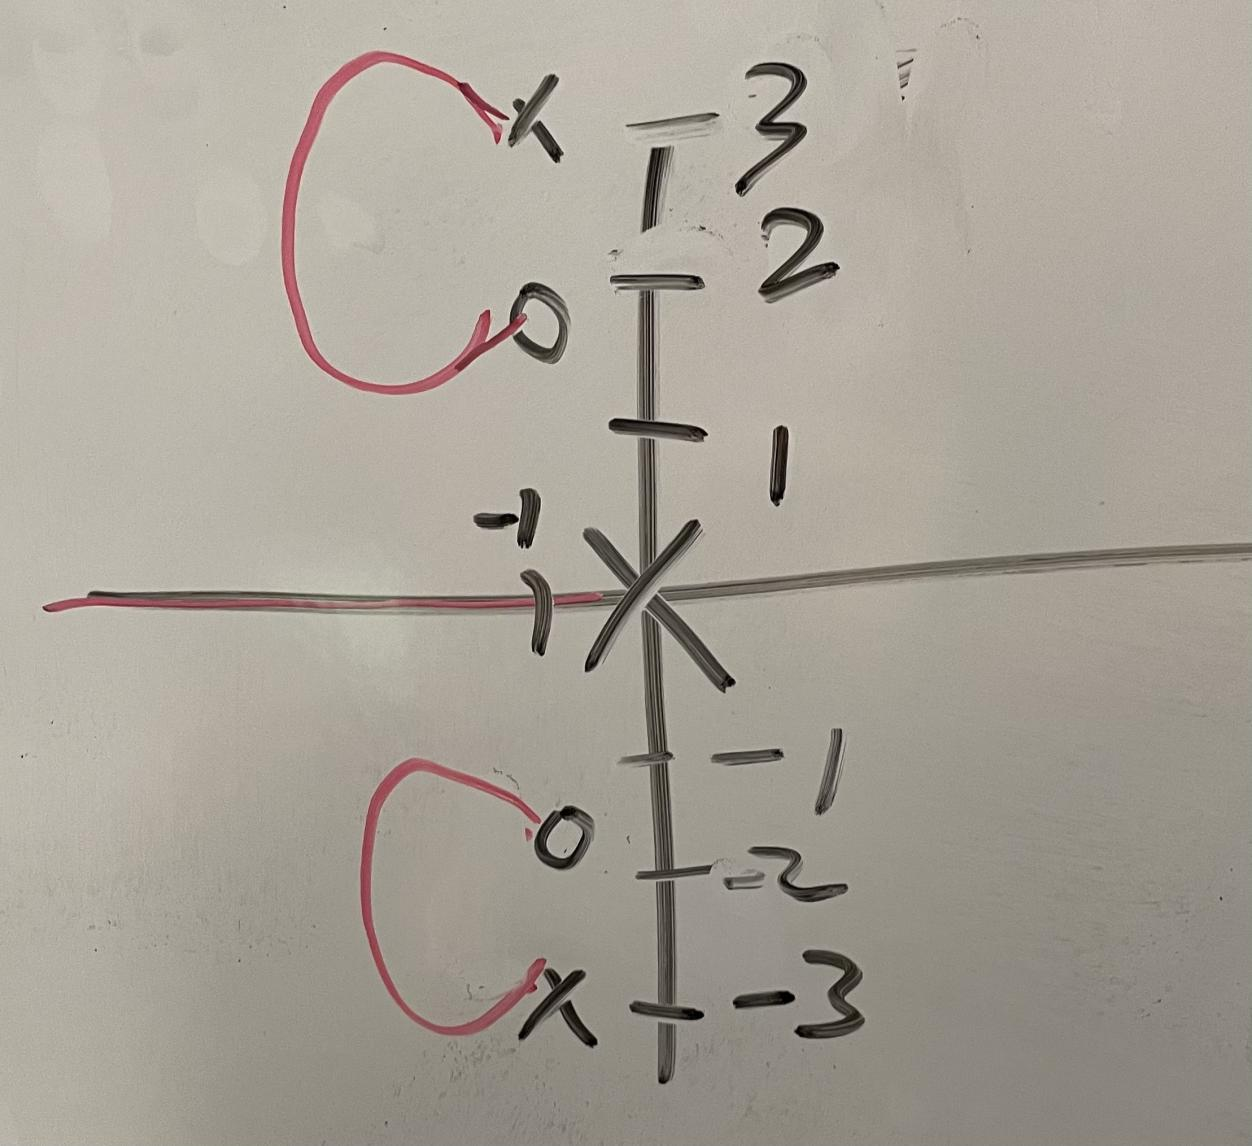
\includegraphics[scale=.15]{Problem1Sketch1.jpg}
\\This coresponds well with the matlab root locus plot:\\
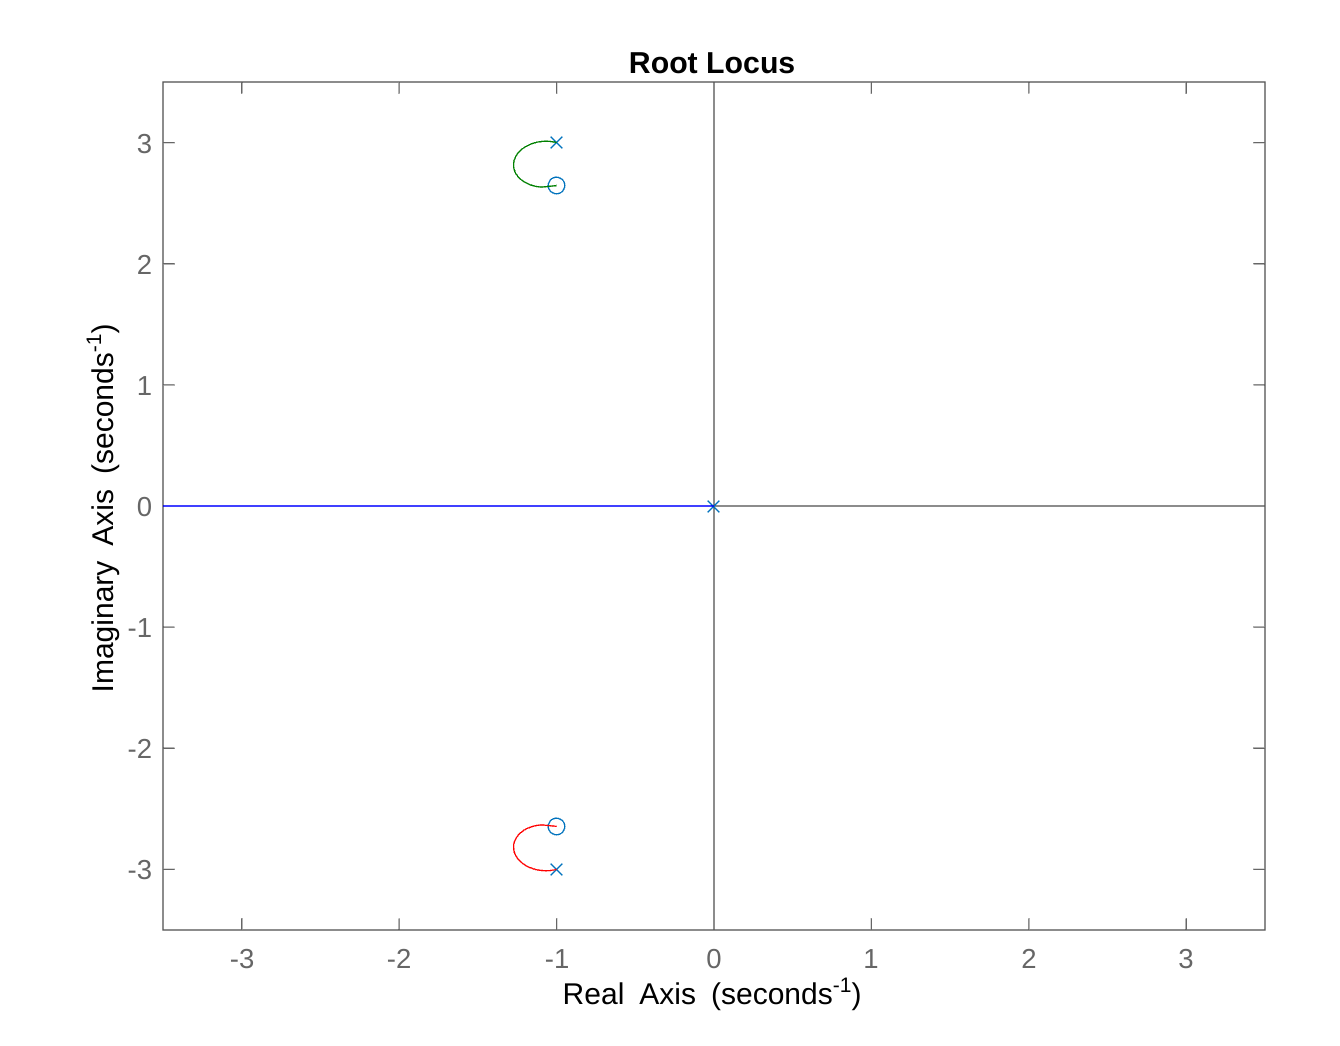
\includegraphics[scale=.15]{Problem1Matlab1.png}
\\That was produced with this code
\begin{verbatim}
sys = tf([1 2 8],[1 2 10 0]);
rlocus(sys)
ylim([-3.5 3.5])
xlim([-3.5 3.5])
\end{verbatim}

\subsection*{(e)}
$L(s)$ has zeros at $\pm j$, and poles at $0$ and $\pm2j$, therefore we have $\alpha=0$
$\phi_{1}=180^{\circ}$, 
And the departure angle for poles $\pm2j$ is $180^{\circ}$, And the arival angle for the zeros $\pm1j$ is $180^{\circ}$\\\\
Therefore the sketch fo the root locus looks like the following
\\
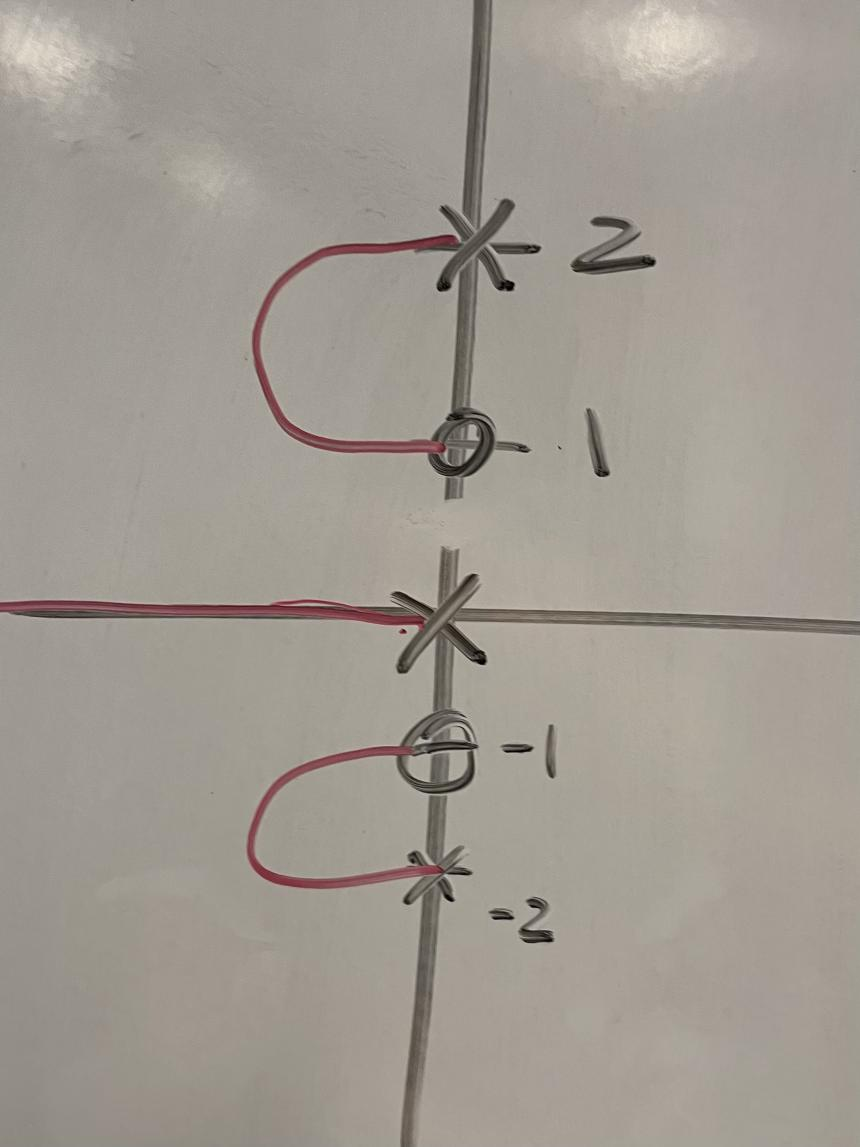
\includegraphics[scale=.15]{Problem1Sketch2.jpg}
\\This coresponds well with the matlab root locus plot:\\
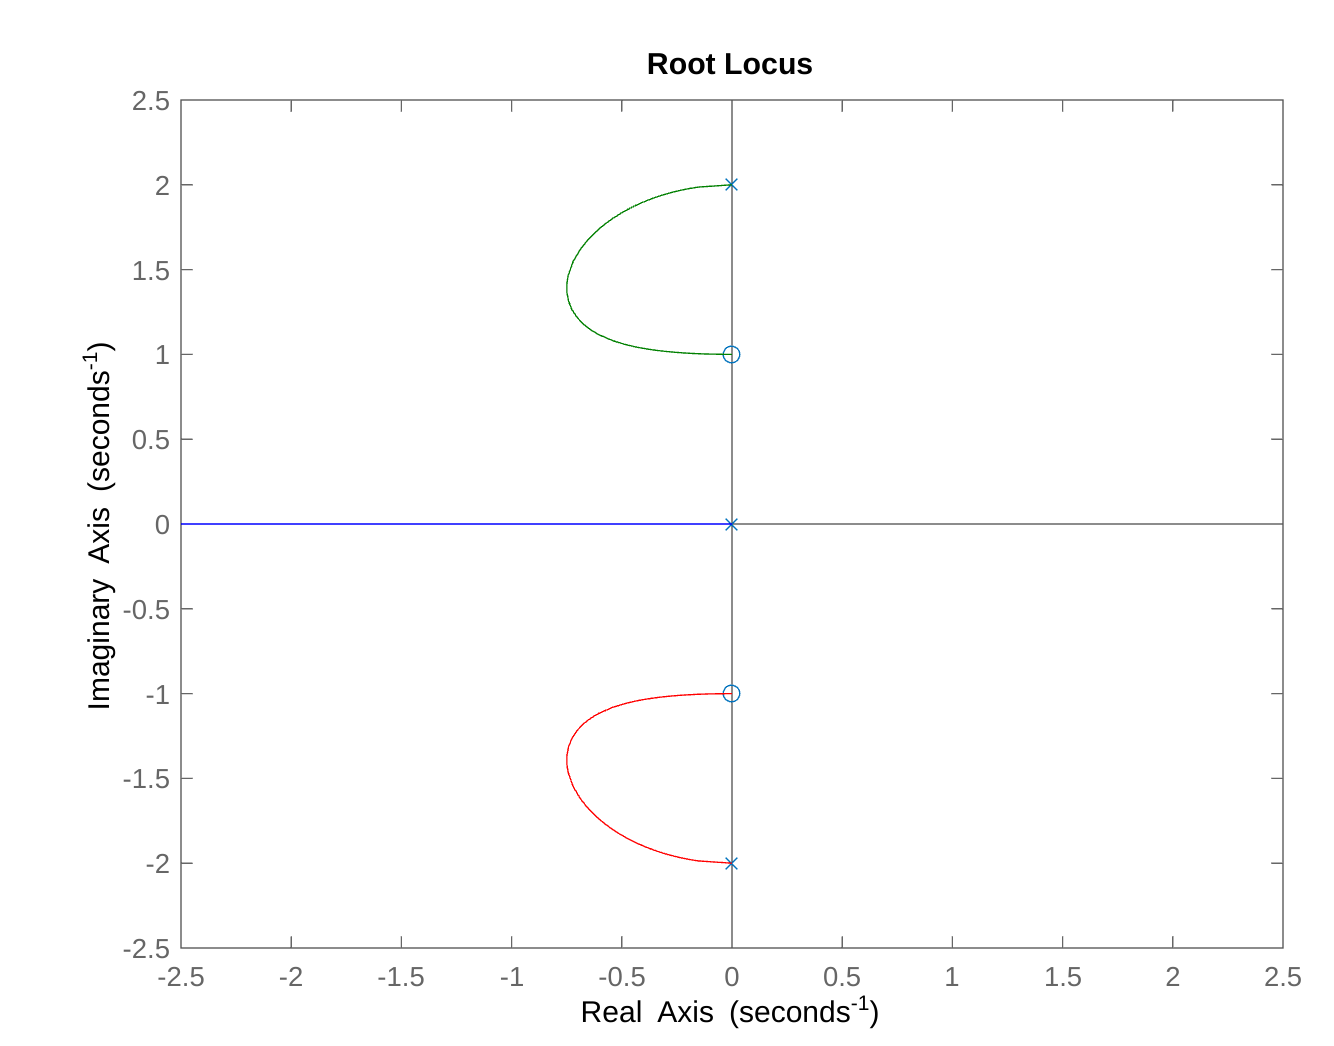
\includegraphics[scale=.15]{Problem1Matlab2.png}
\\That was produced with this code
\begin{verbatim}
sys = tf([1 0 1],[1 0 4 0]);
rlocus(sys)
ylim([-2.5 2.5])
xlim([-2.5 2.5])
\end{verbatim}
\section*{Problem 5.7}
\subsection*{(c)}
This functions has 2 zeros at $-3$ and 5 poles: 2 at $0$, 1 at $-10$, and 2 at $-3\pm4j$
Therefore $\alpha=-3.333$ and and that the three branches intersecting the real axis, intersect at degrees of
$60^{\circ}$, $180^{\circ}$, and $300^{\circ}$,
therefore we have
\\for pole $-10+0j$, departure angle 1: $180^{\circ}$
\\for poles $-3\pm4j$ the departure angles are $\pm13.484^{\circ}$
\\for the dual poles at the $0$ the departure angles are $\pm90^{\circ}$
\\for the dual zeros at $0$ the arrival angles ar $\pm90^{\circ}$
Therefore the sketch fo the root locus looks like the following
\\
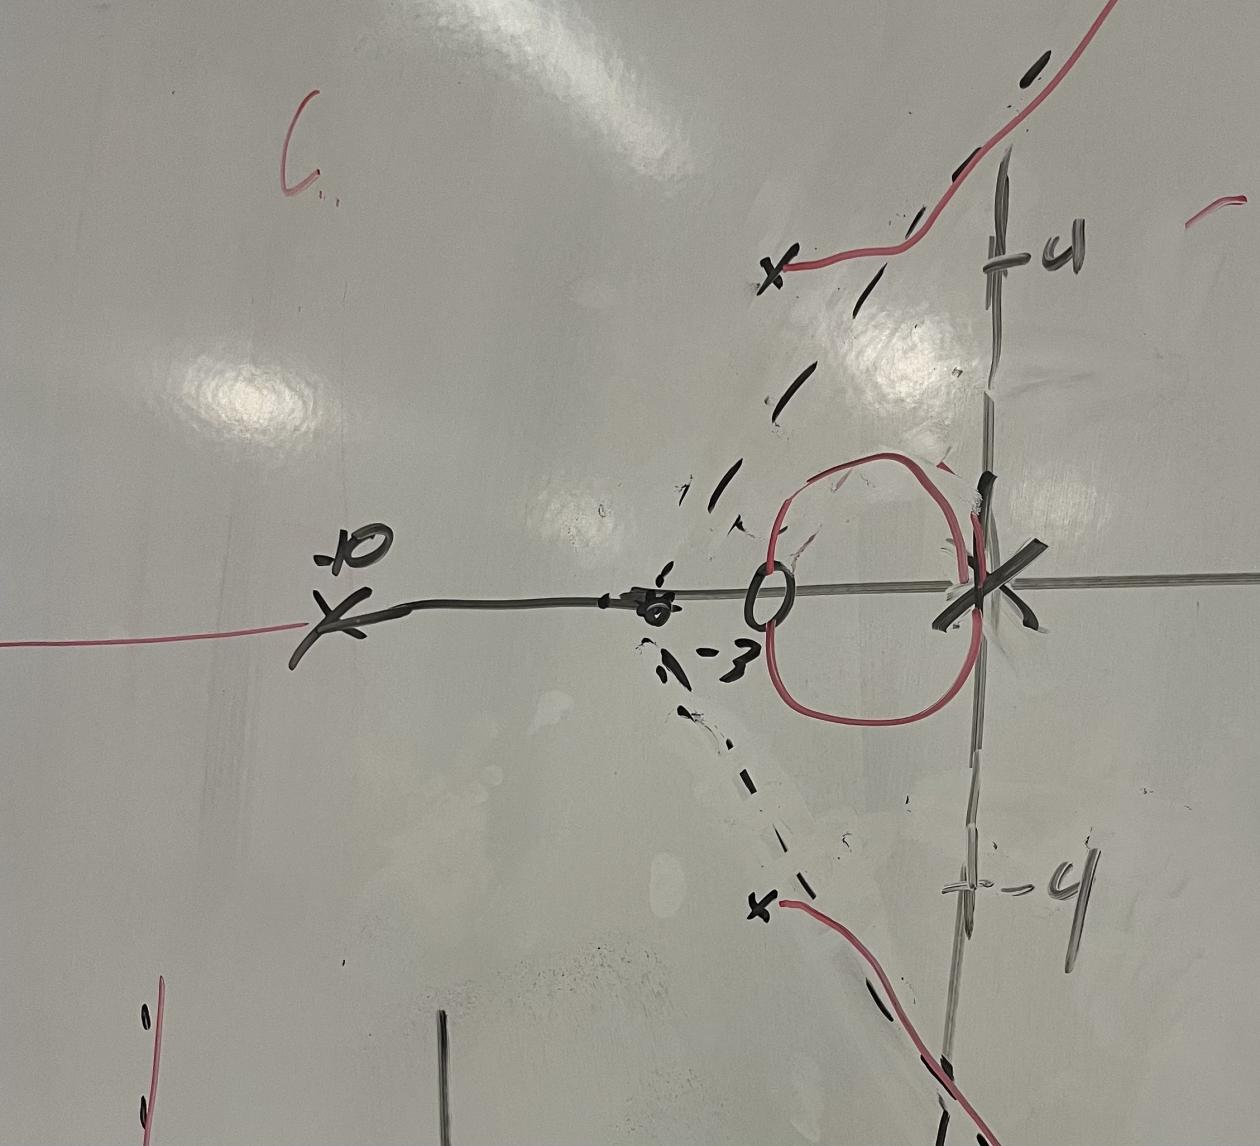
\includegraphics[scale=.15]{Problem2Sketch1.jpg}
\\This coresponds well with the matlab root locus plot:\\
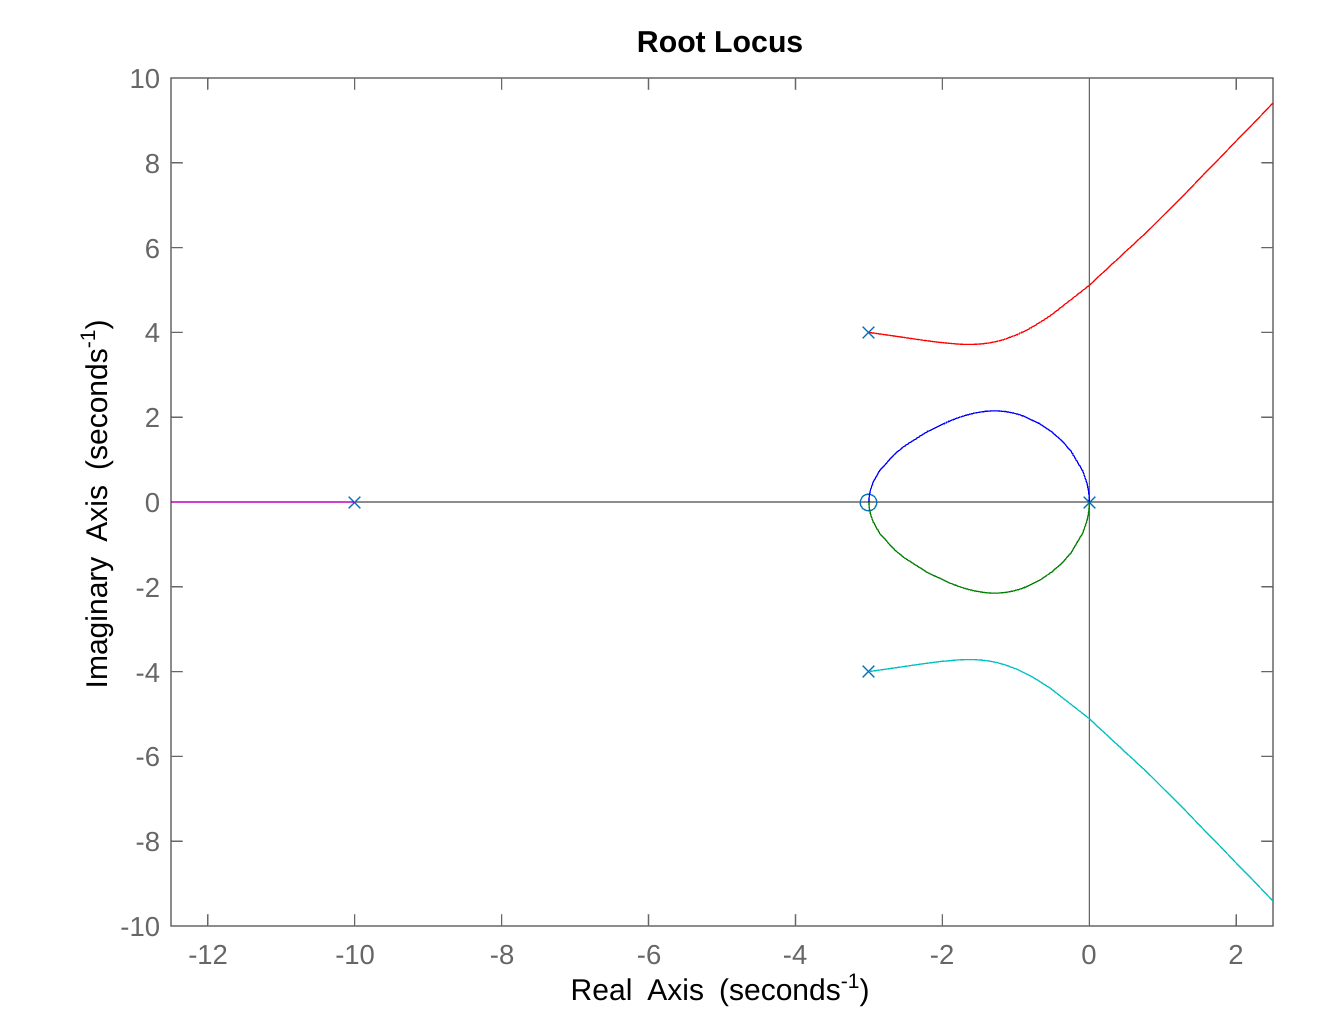
\includegraphics[scale=.2]{Problem2Matlab1.png}
\\That was produced with this code
\begin{verbatim}
sys = tf([1 6 9],[1 16 85 250 0 0]);
rlocus(sys)
ylim([-10 10])
xlim([-12.5 2.5])
\end{verbatim}
\subsection*{(e)}
$L(s)$ had zeros at $-1\pm1j$ and 4 poles, 2 at 0, 1 at $-2$ and $-3$. Therefore we have
$$\alpha=-1.5$$
And there are two lines asymptomatic to this at angles of $\pm90^{\circ}$
\\
We have
\\for pole $-3$, departure angle 1: $0.0^{\circ}$
\\for pole -2, departure angle 1: $180^{\circ}$
\\for pole 0, departure angle 1: $270^{\circ}$
\\for pole 0, departure angle 2: $90^{\circ}$
\\for zero $-1\pm1j$, arrival angle: $\pm71.565^{\circ}$\\
Furthermore from Rule 6 we have that there are mutliple roots where $s=-2.485$, therefore the sketch of the root locus looks like
\\
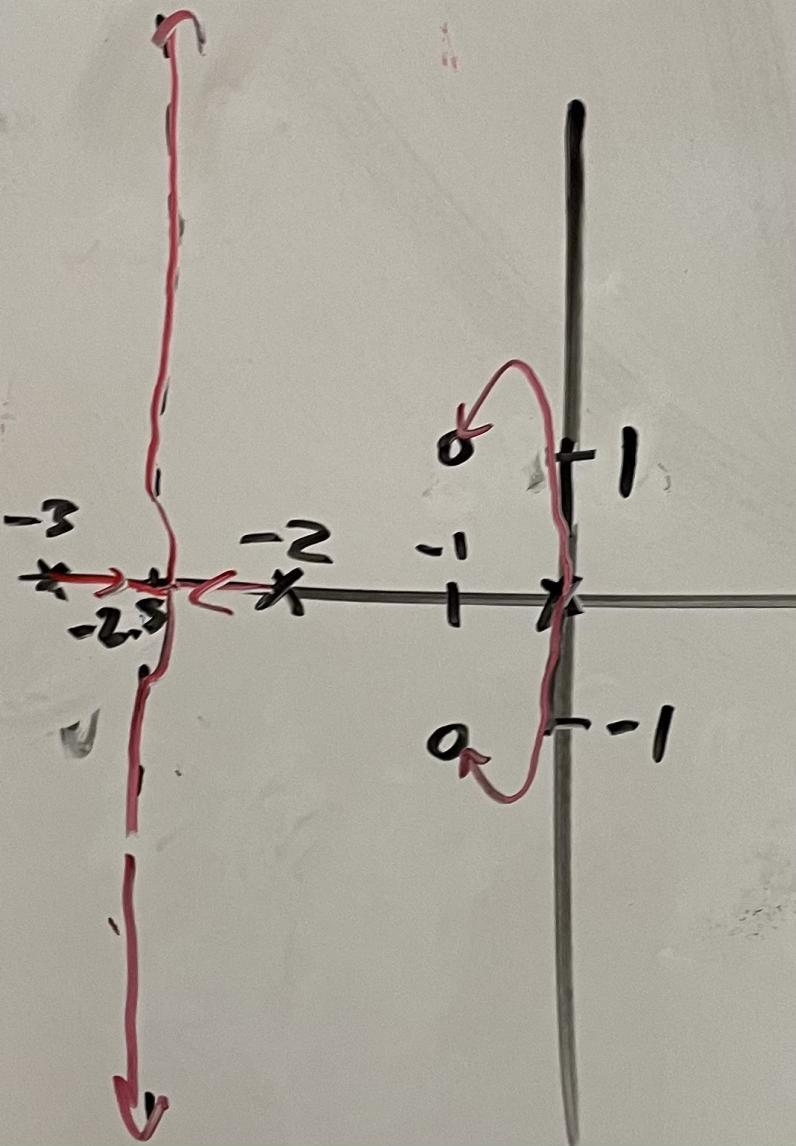
\includegraphics[scale=.15]{Problem2Sketch2.jpg}
\\This coresponds well with the matlab root locus plot:\\
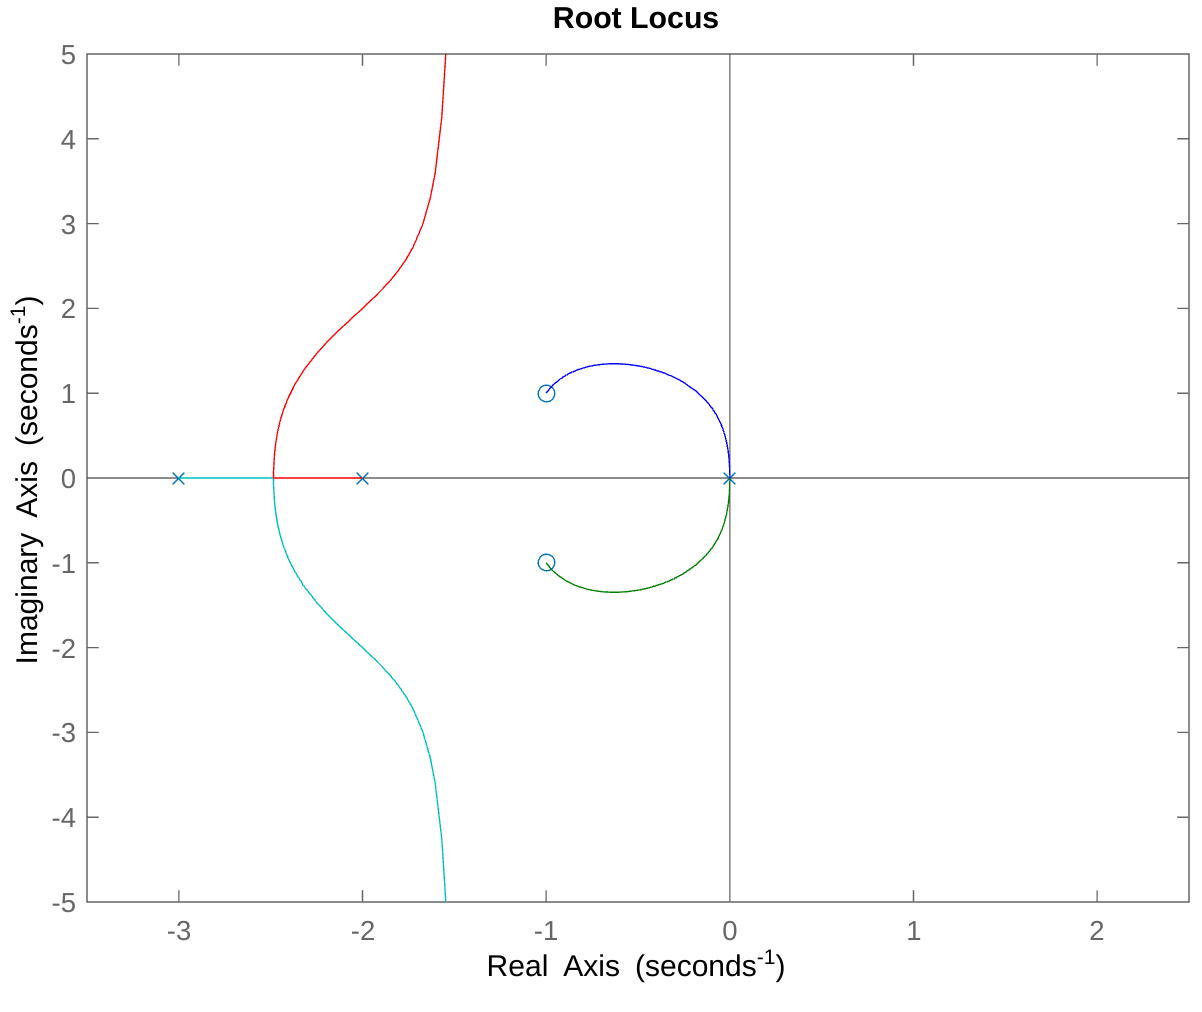
\includegraphics[scale=.2]{Problem2Matlab2.png}
\\That was produced with this code
\begin{verbatim}
sys = tf([1 2 2],[1 5 6 0 0]);
rlocus(sys)
ylim([-5 5])
xlim([-3.5 2.5])
\end{verbatim}
\section*{Problem 5.8}
\subsection*{(e)}
$L(s)$ has a zero at $-2$ and 4 poles, 2 at $-6$, one at $0$, and one at $1$. Therefore,
$$\alpha=-3$$
and three lines are asymptomatic to it at angles of $180$, $60$, and $180$.
For the poles we have that:\\
for pole -6, departure angle 1: $180^{\circ}$
\\for pole -6, departure angle 2: $0^{\circ}$
\\for pole 0, departure angle 1: $0^{\circ}$
\\for pole 1, departure angle 1: $180^{\circ}$
\\and for the zero we have that the angle of arival is $180^{\circ}$,
Furthermore from Rule 6 we have that there are multiple roots where $s=-6,0.488$, therefore the sketch of the root locus looks something like
\\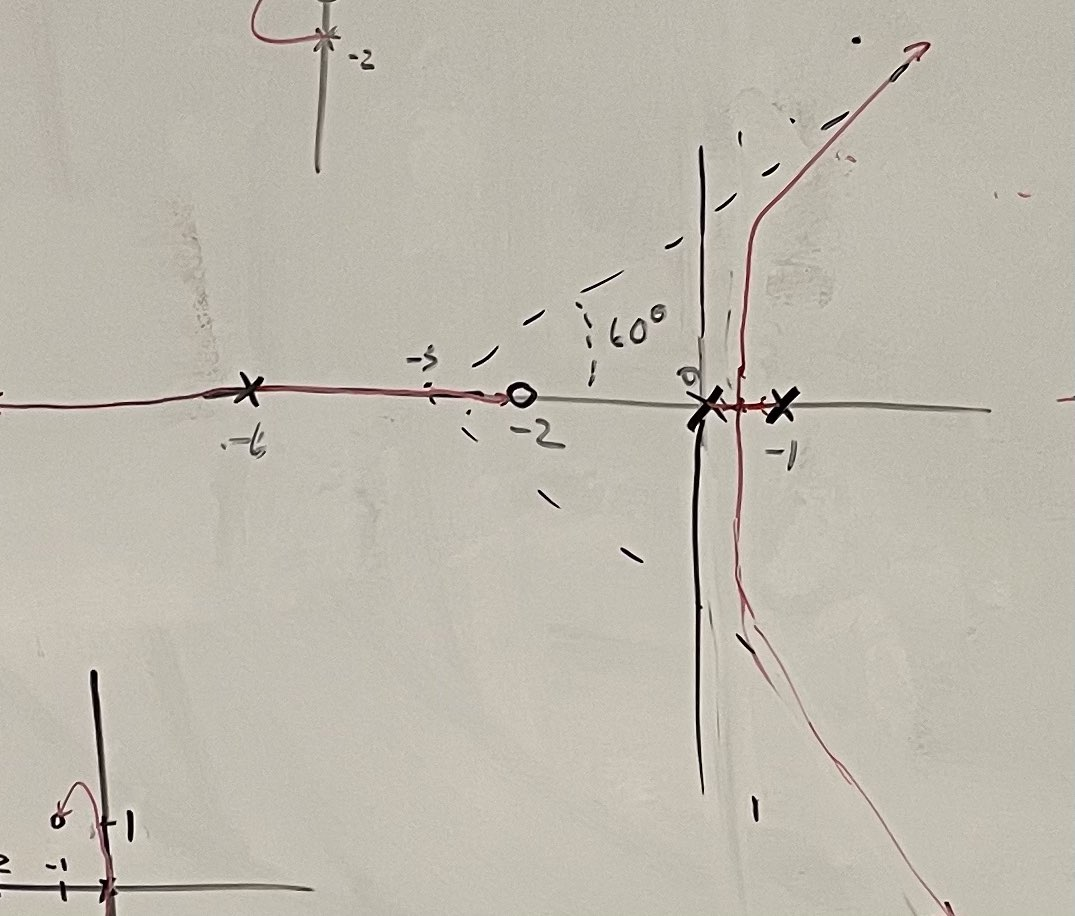
\includegraphics[scale=.15]{Problem3Sketch1.jpg}
\\This coresponds well with the matlab root locus plot:\\
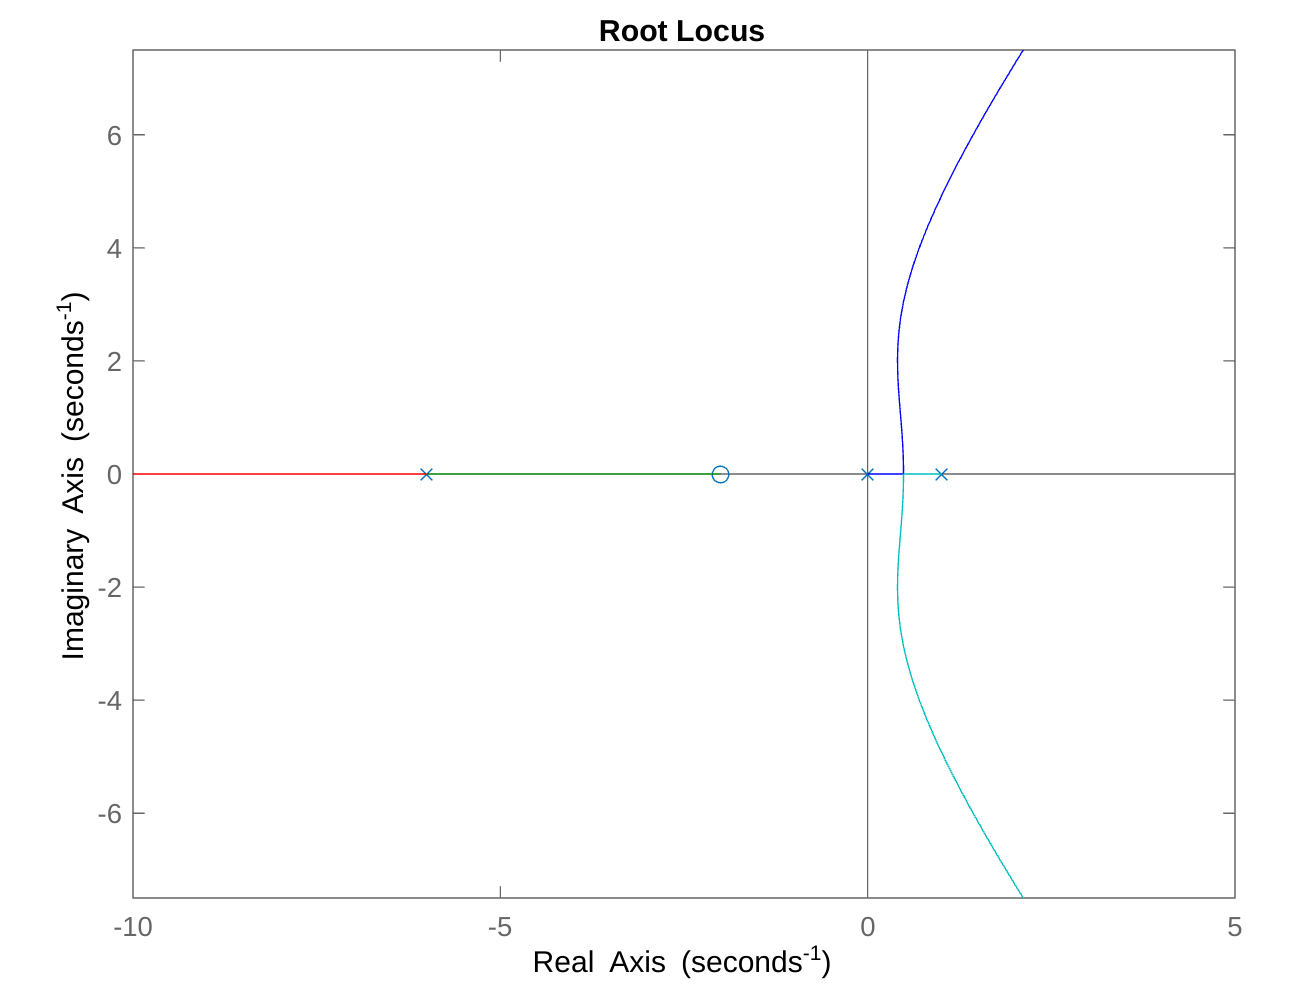
\includegraphics[scale=.2]{Problem3Matlab1.png}
\\That was produced with this code
\begin{verbatim}
sys = tf([1 2],[1 11 24 -36 0]);
rlocus(sys)
ylim([-7.5 7.5])
xlim([-10 5])
\end{verbatim}
\end{document}